% =====================================================================
%  SOUTENANCE — version corrigée
%
%  Corrections apportées à la version précédente
%  ---------------------------------------------
%  1. Les couleurs sont définies AVANT d'être utilisées. `\setbeamercolor{...}{fg=BleuFonce}`
%     précédait `\definecolor{BleuFonce}` : erreur xcolor « Undefined color ».
%  2. `\usepackage{colortbl}` ajouté — `\rowcolor` et `\cellcolor` en dépendent et beamer
%     ne le charge pas.
%  3. Doublons supprimés (tikz, arrows.meta, BleuClair, VertOK, Orange, RougeFaible).
%  4. Fragment orphelin supprimé après « Mesurer par différence » : du texte, `}}`,
%     `\end{center}` et `\end{frame}` traînaient hors de tout `\begin{frame}`.
%  5. Chiffres remis à jour — voir les repères « MAJ » dans le corps.
%  6. Diapos ramenées de 30 à 24 pour tenir en 15 minutes.
%
%  Figures attendues dans le même dossier (ou dans figures/) :
%    courbe_exemple, nettoyage_colonnes, enveloppe_inertie, fig_gains,
%    fig_courbe_393604, fuseau_horaire, flex_avant_apres, profil_flexibilite,
%    fig_flex_reponse, fig_flex_distribution, cma, Mines, Polytech_Nice
% =====================================================================

\documentclass[aspectratio=169,11pt]{beamer}

\usepackage[utf8]{inputenc}
\usepackage[T1]{fontenc}
\usepackage[french]{babel}
\usepackage{graphicx}
\usepackage{colortbl}
\usepackage{tikz}
\usetikzlibrary{arrows.meta, positioning}

\graphicspath{{figures/}{./}}

% ---------- couleurs : définies une seule fois, avant tout usage ----------
\definecolor{BleuFonce}{RGB}{0,74,117}
\definecolor{BleuClair}{RGB}{222,235,247}
\definecolor{VertOK}{RGB}{198,239,206}
\definecolor{RougeFaible}{RGB}{255,199,206}
\definecolor{Orange}{RGB}{230,145,56}
\definecolor{GrisLeger}{RGB}{242,242,242}
\definecolor{JauneMoy}{RGB}{255,235,156}

\usetheme{default}
\setbeamercolor{title}{fg=BleuFonce}
\setbeamercolor{subtitle}{fg=black}
\setbeamercolor{author}{fg=black}
\setbeamercolor{institute}{fg=black!70}
\setbeamercolor{structure}{fg=BleuFonce}
\setbeamercolor{frametitle}{fg=BleuFonce}
\setbeamerfont{frametitle}{size=\large,series=\bfseries}
\setbeamerfont{title}{size=\Large,series=\bfseries}
\setbeamerfont{subtitle}{size=\small,shape=\itshape}
\setbeamertemplate{navigation symbols}{}
\setbeamertemplate{itemize item}{\color{Orange}$\blacktriangleright$}

\tikzset{etape/.style={rectangle, rounded corners=3pt,
  draw=BleuFonce, fill=BleuClair, line width=0.7pt,
  text width=1.9cm, align=center, minimum height=0.9cm, font=\tiny}}
\tikzset{etapeo/.style={etape, draw=Orange, fill=Orange!15}}
\tikzset{final/.style={etape, draw=BleuFonce, fill=BleuFonce,
  text=white, font=\tiny\bfseries, text width=2.1cm}}
\tikzset{fl/.style={-{Stealth[length=1.6mm]}, draw=BleuFonce!70, line width=0.6pt}}

\newcommand{\encadre}[2][BleuClair]{%
  \begin{center}\colorbox{#1}{\parbox{0.88\textwidth}{\centering\vspace{0.4em}#2\vspace{0.4em}}}\end{center}}

\title{Apprentissage automatique appliqué au gisement de flexibilité électrique
résidentielle}
\subtitle{Prédiction de la consommation et estimation du gisement par simulation
contrefactuelle}
\author{Boubaker Amdyoun}
\institute{Polytech Nice Sophia --- SI4\\[2pt]
Stage au Centre de Mathématiques Appliquées, MINES Paris--PSL\\[2pt]
Tuteurs : Damien Corral et Gilles Guerassimoff}
\date{Septembre 2026}
\titlegraphic{%
  \IfFileExists{Mines.png}{\includegraphics[height=1.1cm]{Mines.png}}{}%
  \hspace{1.5cm}%
  \IfFileExists{Polytech_Nice.png}{\includegraphics[height=1.1cm]{Polytech_Nice.png}}{}}

\begin{document}

\begin{frame}[plain]
\titlepage
\end{frame}

% ==================== 1 ====================
\begin{frame}{Où j'ai effectué ce stage}
\begin{columns}[T]
\begin{column}{0.48\textwidth}
\vspace{1.2em}
\begin{itemize}\setlength{\itemsep}{0.9em}
  \item \textbf{Centre de Mathématiques Appliquées}, MINES Paris--PSL
  \item À \textbf{Valbonne}, sur la technopole de Sophia Antipolis
  \item Un \textbf{laboratoire de recherche} : deux chercheurs, trois stagiaires
\end{itemize}
\vspace{1em}
{\small Une réunion d'équipe de deux heures chaque semaine.}
\end{column}
\begin{column}{0.48\textwidth}
\centering
\IfFileExists{cma.jpg}{\includegraphics[width=\linewidth]{cma.jpg}}
  {\framebox[\linewidth]{\rule{0pt}{4.2cm}\parbox{5cm}{\centering Photo du CMA\\
   \small (à insérer : \texttt{cma.jpg})}}}
\end{column}
\end{columns}
\end{frame}

% ==================== 2 ====================
% MAJ : les diapos « Le projet FlexiMax » et « Mon volet » ont été fusionnées.
\begin{frame}{Le projet FlexiMax, et mon volet}

\begin{itemize}\setlength{\itemsep}{0.5em}
  \item Financé par \textbf{France 2030}, opéré par l'\textsc{Ademe}
  \item Objectif du consortium : \textbf{piloter} les charges en temps réel
\end{itemize}

\vspace{0.8em}
\begin{center}
{\large Ma question : \textbf{où se situe la flexibilité ?}}
\end{center}

\vspace{0.5em}
\begin{columns}[T]
\begin{column}{0.3\textwidth}\centering
\colorbox{BleuClair}{\parbox{0.92\textwidth}{\centering\vspace{0.4em}
Dans quels\\\textbf{logements}\vspace{0.4em}}}
\end{column}
\begin{column}{0.3\textwidth}\centering
\colorbox{BleuClair}{\parbox{0.92\textwidth}{\centering\vspace{0.4em}
À quelles\\\textbf{heures}\vspace{0.4em}}}
\end{column}
\begin{column}{0.3\textwidth}\centering
\colorbox{BleuClair}{\parbox{0.92\textwidth}{\centering\vspace{0.4em}
Portée par quels\\\textbf{usages}\vspace{0.4em}}}
\end{column}
\end{columns}

\vspace{0.9em}
\encadre[Orange!15]{Les résultats décrivent un \textbf{potentiel}.\\
Ils ne mesurent pas un effacement réalisé.}
\end{frame}

% ==================== 3 ====================
% Une étape du plan : \planetape{numéro}{titre}{sous-titre}{couleur de fond}
\newcommand{\planetape}[4]{%
  \begin{tikzpicture}
    \node[rectangle, rounded corners=4pt, fill=#4, inner sep=0pt,
          minimum height=1.15cm, text width=0.90\textwidth] (band) {};
    \node[circle, fill=BleuFonce, text=white, font=\bfseries\normalsize,
          minimum size=0.72cm, anchor=west] (num) at ([xshift=0.45cm]band.west) {#1};
    \node[anchor=west, align=left, text width=0.72\textwidth]
         at ([xshift=0.35cm]num.east)
         {\textbf{#2}\\[0.15em]{\small #3}};
  \end{tikzpicture}\\[0.35em]}

\begin{frame}{Plan de l'exposé}
\vspace{0.6em}
\centering
\planetape{1}{Les données}{Un parc simulé plutôt qu'un parc mesuré}{BleuClair}
\planetape{2}{Les variables}{Faire entrer la physique avant le modèle}{GrisLeger}
\planetape{3}{Les modèles}{De la consommation annuelle à la courbe horaire}{BleuClair}
\planetape{4}{Le gisement}{L'estimer, puis le valider}{Orange!18}
\end{frame}

% ==================== 4 ====================
% MAJ : « La volumétrie » fusionnée ici.
\begin{frame}{ResStock : simuler plutôt que mesurer}
\vspace{0.4em}
\centering
\begin{tikzpicture}[node distance=0.35cm and 0.55cm]
\node[etape] (enq) {Enquêtes publiques};
\node[etape, right=of enq] (ech) {Échantillonnage par quotas};
\node[final, right=of ech] (parc) {549\,971 logements};
\node[etape, right=of parc] (sim) {Simulation EnergyPlus};
\node[etapeo, above right=0.25cm and 0.55cm of sim] (meta) {Métadonnées 771 attributs};
\node[etapeo, below right=0.25cm and 0.55cm of sim] (ts) {Séries 15 min};
\draw[fl] (enq)--(ech); \draw[fl] (ech)--(parc); \draw[fl] (parc)--(sim);
\draw[fl] (sim)--(meta); \draw[fl] (sim)--(ts);
\end{tikzpicture}

\vspace{1em}
\begin{columns}[c]
\begin{column}{0.31\textwidth}\centering
\colorbox{BleuClair}{\parbox{0.92\textwidth}{\centering\vspace{0.4em}
{\large\textbf{549 971}}\\[0.2em]{\small logements}\vspace{0.4em}}}
\end{column}
\begin{column}{0.31\textwidth}\centering
\colorbox{BleuClair}{\parbox{0.92\textwidth}{\centering\vspace{0.4em}
{\large\textbf{771}}\\[0.2em]{\small attributs}\vspace{0.4em}}}
\end{column}
\begin{column}{0.31\textwidth}\centering
\colorbox{Orange!20}{\parbox{0.92\textwidth}{\centering\vspace{0.4em}
{\large\textbf{35 040}}\\[0.2em]{\small pas de temps par bâtiment}\vspace{0.4em}}}
\end{column}
\end{columns}

\vspace{0.8em}
{\small\centering Pour chaque logement, la courbe de charge \emph{et} les
caractéristiques qui l'expliquent.\par}
\end{frame}

% ==================== 5 ====================
\begin{frame}{La décomposition par usage}
\begin{columns}[T]
\begin{column}{0.36\textwidth}
\vspace{1.5em}
\begin{itemize}\setlength{\itemsep}{0.9em}
  \item Chauffage, climatisation, eau chaude, électroménager\dots
  \item Séparés, heure par heure
  \item C'est ce qui rend le gisement \textbf{quantifiable}
\end{itemize}
\end{column}
\begin{column}{0.62\textwidth}\centering
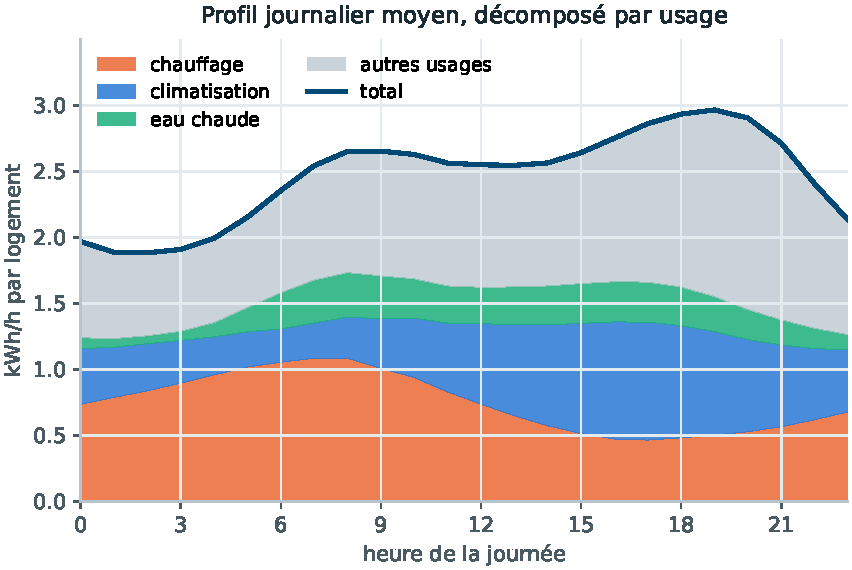
\includegraphics[width=\linewidth]{courbe_exemple.png}
\end{column}
\end{columns}
\end{frame}

% ==================== 5bis ====================
% AJOUT : à quoi ressemble le parc, côté métadonnées.
\begin{frame}{Sur quoi je travaille : les logements}
\vspace{0.2em}
\centering
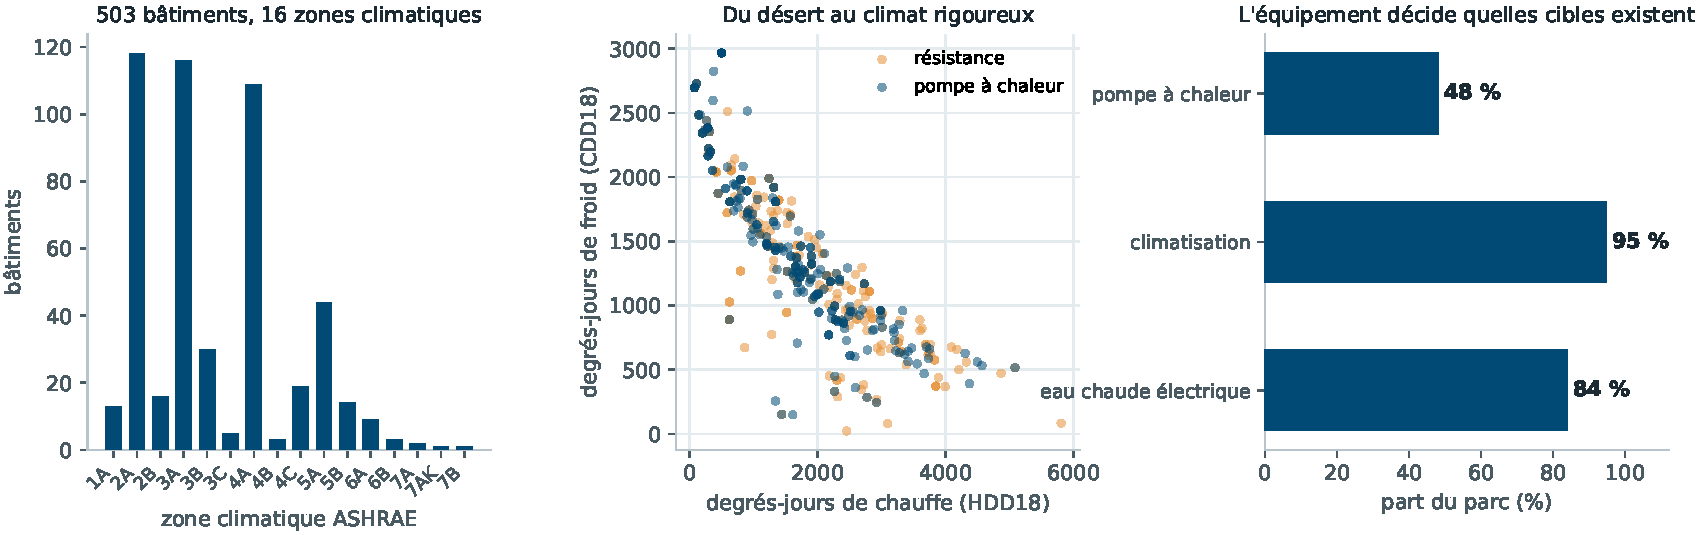
\includegraphics[width=\textwidth]{parc_metadonnees.png}

\vspace{0.5em}
\begin{itemize}\setlength{\itemsep}{0.3em}
  \item \textbf{16 zones climatiques}, du désert de l'Arizona au Colorado à
  $-22$\,°C : le parc n'est pas concentré sur un seul climat
  \item \textbf{48 \%} de pompes à chaleur --- deux populations qui consomment
  d'un facteur trois pour le même besoin
  \item 5 \% sans climatisation, 16 \% sans eau chaude électrique : leur
  consommation de cet usage est \textbf{strictement nulle}, et le modèle doit le
  savoir
\end{itemize}
\end{frame}

% ==================== 5ter ====================
% AJOUT : à quoi ressemblent les courbes.
\begin{frame}{Sur quoi je travaille : les courbes}
\vspace{0.2em}
\centering
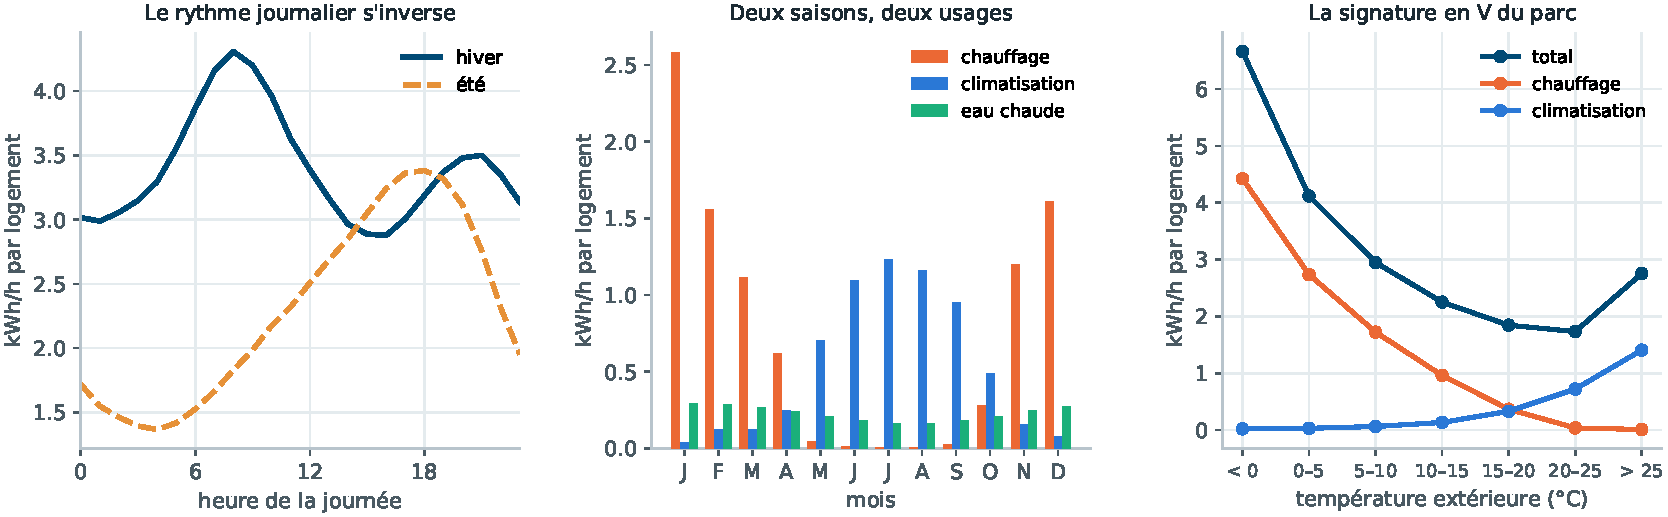
\includegraphics[width=\textwidth]{parc_timeseries.png}

\vspace{0.5em}
\begin{itemize}\setlength{\itemsep}{0.3em}
  \item Le rythme journalier \textbf{s'inverse} d'une saison à l'autre : pointe
  du matin en hiver, pointe de fin d'après-midi en été
  \item Chauffage et climatisation ne se recouvrent presque pas --- ce sont deux
  gisements \textbf{disjoints dans le temps}
  \item La \textbf{signature en V} : c'est cette dépendance à la température que
  le modèle doit apprendre
\end{itemize}
\end{frame}

% ==================== 6 ====================
% MAJ : « Le nettoyage » et « Encoder : ce qui n'allait pas » fusionnées.
\begin{frame}{Du brut à l'exploitable : 771 $\rightarrow$ 165}
\begin{columns}[T]
\begin{column}{0.42\textwidth}
\vspace{0.8em}
\begin{itemize}\setlength{\itemsep}{0.7em}
  \item Attributs \textbf{constants}, \textbf{redondants}, ou vides
  \item Puis un \textit{one-hot} générique : des dizaines de variables pour une
  même réalité thermique
\end{itemize}
\vspace{0.6em}
{\footnotesize Remis en cause \textbf{en réunion}, grâce au regard métier de mes
tuteurs.}
\end{column}
\begin{column}{0.56\textwidth}\centering
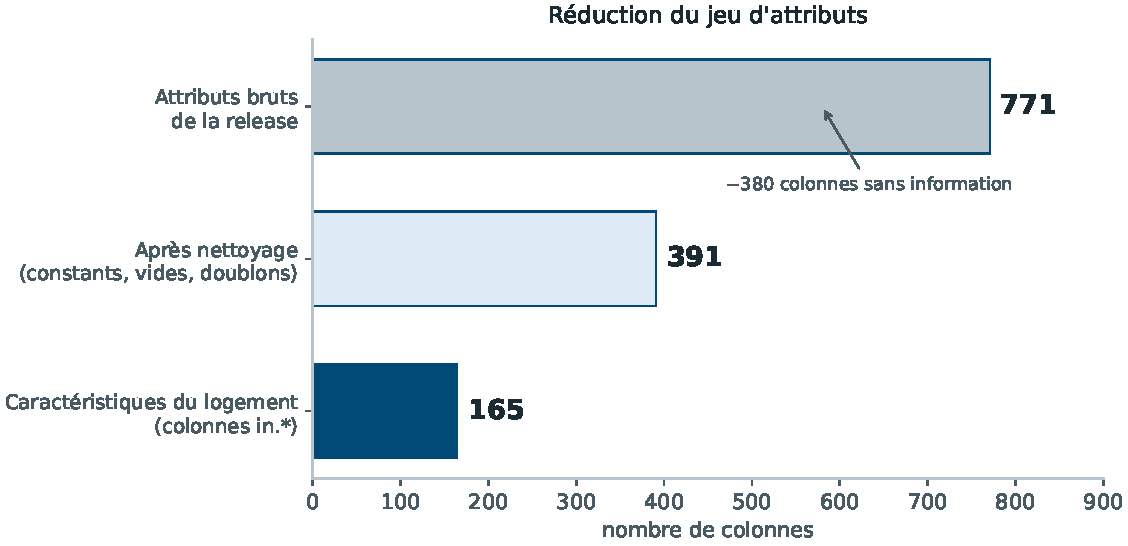
\includegraphics[width=\linewidth]{nettoyage_colonnes.png}
\end{column}
\end{columns}
\vspace{0.3em}
\encadre[Orange!15]{Ne pas laisser le modèle redécouvrir ce que la physique
établit déjà.}
\end{frame}

% ==================== 7 ====================
\begin{frame}{Ce qui fait la thermique d'un logement}
\centering
\begin{tikzpicture}[scale=0.68, line width=0.7pt,
  lab/.style={font=\scriptsize, align=left},
  fl2/.style={-{Stealth[length=2mm]}, BleuFonce, line width=0.7pt}]

\fill[GrisLeger] (-0.5,-0.2) rectangle (6.0,0);
\fill[BleuClair] (0,0) rectangle (4,2.6);
\draw[BleuFonce] (0,0) rectangle (4,2.6);
\fill[BleuClair!55] (4,0) -- (5.2,0.8) -- (5.2,3.4) -- (4,2.6) -- cycle;
\draw[BleuFonce] (4,0) -- (5.2,0.8) -- (5.2,3.4) -- (4,2.6) -- cycle;
\fill[Orange!25] (0,2.6) -- (2,3.9) -- (4,2.6) -- cycle;
\draw[BleuFonce] (0,2.6) -- (2,3.9) -- (4,2.6) -- cycle;
\fill[Orange!45] (2,3.9) -- (4,2.6) -- (5.2,3.4) -- (3.2,4.7) -- cycle;
\draw[BleuFonce] (2,3.9) -- (4,2.6) -- (5.2,3.4) -- (3.2,4.7) -- cycle;
\fill[white] (0.5,1.2) rectangle (1.3,2.0);
\draw[BleuFonce] (0.5,1.2) rectangle (1.3,2.0);
\fill[white] (2.7,1.2) rectangle (3.5,2.0);
\draw[BleuFonce] (2.7,1.2) rectangle (3.5,2.0);
\fill[BleuFonce!25] (1.75,0) rectangle (2.45,1.5);
\draw[BleuFonce] (1.75,0) rectangle (2.45,1.5);

\node[lab, anchor=east] (Lmur) at (-1.0,2.3) {Murs\\$R_{\text{mur}}$};
\draw[fl2] (Lmur.east) -- (0.15,2.3);
\node[lab, anchor=east] (Lfen) at (-1.0,1.55) {Fenêtres\\$U_{\text{fen}}$, SHGC};
\draw[fl2] (Lfen.east) -- (0.45,1.6);
\node[lab, anchor=east] (Lsol) at (-1.0,0.4) {Plancher\\$R_{\text{sol}}$};
\draw[fl2] (Lsol.east) -- (0.4,0.1);
\node[lab, anchor=west] (Ltoit) at (6.1,4.6) {Toiture\\$R_{\text{toit}}$};
\draw[fl2] (Ltoit.west) -- (4.4,4.2);
\node[lab, anchor=west] (Linf) at (6.1,2.6) {Infiltrations\\ACH50 $\rightarrow H_{ve}$};
\draw[fl2] (Linf.west) -- (5.3,2.4);
\node[lab, anchor=west] (Liner) at (6.1,1.0) {Inertie du bâti\\$C$};
\draw[fl2] (Liner.west) -- (5.0,1.2);

\fill[JauneMoy] (0.4,4.4) circle (0.32);
\foreach \a in {0,45,...,315}
  \draw[JauneMoy!80!black, line width=0.6pt] (\a:0.42) ++(0.4,4.4) -- ++(\a:0.18);
\draw[-{Stealth[length=2mm]}, JauneMoy!70!black, line width=0.9pt]
  (0.9,4.1) -- (2.6,2.2);
\node[lab, anchor=south west, text=JauneMoy!60!black] at (1.2,3.4) {Apports solaires};
\end{tikzpicture}

\vspace{0.4em}
\small Une quarantaine d'attributs bruts, ramenés à \textbf{cinq grandeurs} :
$UA$, $H_{ve}$, $C$, $A_{\text{solaire}}$, compacité.
\end{frame}

% ==================== 8 ====================
\begin{frame}{La constante de temps : pourquoi un effacement est possible}
\centering
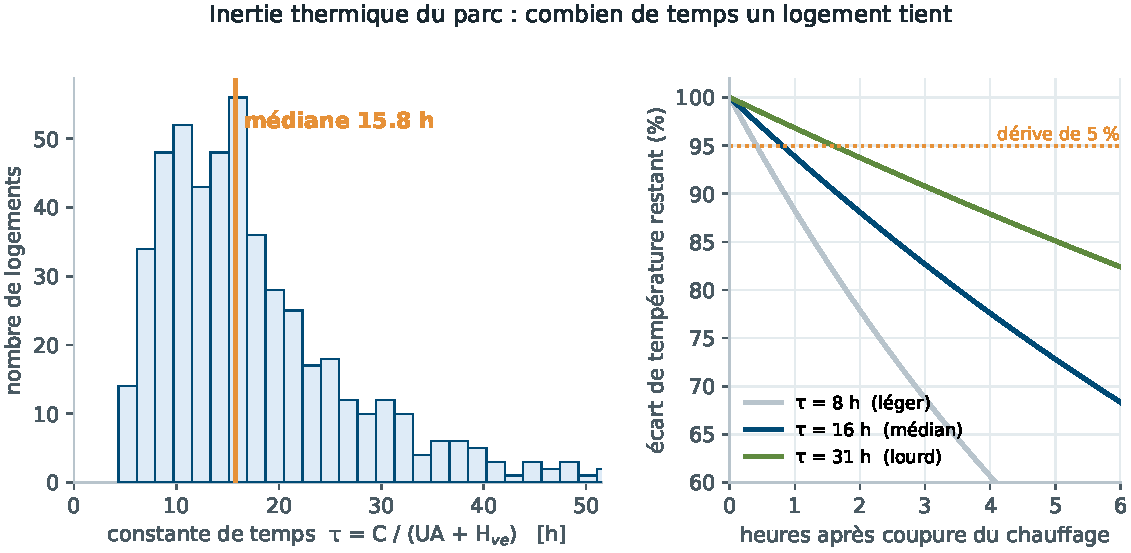
\includegraphics[width=0.94\linewidth]{enveloppe_inertie.png}

\vspace{0.4em}
\encadre[VertOK]{$\tau = C/(UA + H_{ve})$ --- médiane \textbf{15,8 h}\\[0.2em]
\small Un logement peut voir son chauffage réduit une à deux heures sans écart
sensible de température.}
\end{frame}

% ==================== 9 ====================
% MAJ : « Pourquoi LightGBM » et « Le modèle annuel » fusionnées.
\begin{frame}{Le modèle annuel}
\vspace{0.4em}
\begin{itemize}\setlength{\itemsep}{0.6em}
  \item Prédit la consommation \textbf{annuelle} à partir des seules
  caractéristiques du logement --- quatre cibles : total, chauffage,
  climatisation, eau chaude
  \item \textbf{LightGBM} : des arbres qui corrigent successivement l'erreur du
  précédent. Adapté aux tableaux hétérogènes, sans normalisation
  \item Sous-parc filtré : maisons de plain-pied \textbf{tout-électriques}, sans
  véhicule électrique, piscine ni photovoltaïque
  \item Découpage \textbf{stratifié} par zone climatique
\end{itemize}
\vspace{0.5em}
\encadre{\small 64 062 logements --- 41 000 en apprentissage, 12 813 en test.}
\end{frame}

% ==================== 10 ====================
\begin{frame}{Le levier décisif : le système de chauffage}
\vspace{0.2em}
\begin{itemize}\setlength{\itemsep}{0.4em}
  \item Les 47 variables d'origine ne contenaient \textbf{ni} le type de
  chauffage, \textbf{ni} son rendement, \textbf{ni} le combustible
  \item Le modèle ne pouvait pas distinguer une pompe à chaleur d'un convecteur
\end{itemize}

\vspace{0.7em}
\centering\small
\renewcommand{\arraystretch}{1.3}
\begin{tabular}{@{}l c c@{}}
\rowcolor{BleuFonce}
\textcolor{white}{\textbf{À besoin thermique égal}} &
\textcolor{white}{\textbf{Consommation}} &
\textcolor{white}{\textbf{Biais du modèle}} \\
\rowcolor{RougeFaible} Convecteur électrique & 9\,854 kWh/an & $-16$ \% \\
\rowcolor{VertOK} Pompe à chaleur & 3\,175 kWh/an & $+37$ \% \\
\end{tabular}

\vspace{0.9em}
\encadre[Orange!18]{Trois colonnes ajoutées --- présence d'une PAC, COP
saisonnier, mini-split ---\\[0.2em]
\textbf{$+0{,}153$ de $R^2$ sur le chauffage}.}
\end{frame}

% ==================== 11 ====================
\begin{frame}{Performance du modèle annuel}
\vspace{0.4em}
\centering\small
\renewcommand{\arraystretch}{1.35}
\begin{tabular}{@{}l c c c c@{}}
\rowcolor{BleuFonce}
\textcolor{white}{\textbf{Usage}} & \textcolor{white}{\textbf{47 variables}} &
\textcolor{white}{\textbf{61 variables}} & \textcolor{white}{\textbf{$\Delta$}} &
\textcolor{white}{\textbf{RMSE}} \\
\rowcolor{GrisLeger} Total & 0,886 & 0,943 & $+0{,}057$ & 2\,377 \\
Chauffage & 0,800 & 0,953 & \cellcolor{VertOK}$\mathbf{+0{,}153}$ & 1\,649 \\
\rowcolor{GrisLeger} Climatisation & 0,916 & 0,957 & $+0{,}041$ & 645 \\
Eau chaude & 0,975 & 0,975 & $+0{,}000$ & 241 \\
\end{tabular}

\vspace{0.5em}
{\footnotesize RMSE en kWh/an --- jeu de test, \textbf{12 813 logements}}

\vspace{0.8em}
\encadre{\small L'enrichissement des variables a plus apporté que tout réglage
d'hyperparamètre.}
\end{frame}

% ==================== 12 ====================
\begin{frame}{Un piège évité}
\vspace{0.3em}
\encadre[RougeFaible]{L'arrêt anticipé se faisait sur le \textbf{jeu de test}.\\[0.2em]
\small Le nombre d'arbres était donc choisi sur les données servant à juger le
modèle.}

\vspace{0.5em}
\begin{itemize}\setlength{\itemsep}{0.4em}
  \item Score affiché par l'ancien fichier : \textbf{0,949} --- un modèle honnête
  plafonne à \textbf{0,886}
  \item Les niveaux transmis au réseau sont désormais produits \textbf{hors
  échantillon}, en cinq plis
\end{itemize}

\vspace{0.7em}
\centering\small
\renewcommand{\arraystretch}{1.25}
\begin{tabular}{@{}l c c c c@{}}
\rowcolor{BleuFonce}
\textcolor{white}{\textbf{Jeu}} & \textcolor{white}{\textbf{total}} &
\textcolor{white}{\textbf{chauffage}} & \textcolor{white}{\textbf{clim}} &
\textcolor{white}{\textbf{eau chaude}} \\
\rowcolor{GrisLeger} Test --- 12 813 & 0,9427 & 0,9534 & 0,9570 & 0,9750 \\
Validation croisée --- 64 062 & 0,9415 & 0,9508 & 0,9552 & 0,9809 \\
\rowcolor{VertOK} Écart & 0,001 & 0,003 & 0,002 & 0,006 \\
\end{tabular}

\vspace{0.5em}
{\small Les deux coïncident : le fichier n'a plus rien d'optimiste.}
\end{frame}

% ==================== 13 ====================
% MAJ : « lit la journée » -> « lit la semaine » (la fenêtre fait 168 h).
\begin{frame}{Deux modèles chaînés}
\vspace{0.3em}
\centering
\begin{tikzpicture}[scale=0.92, transform shape, node distance=0.32cm and 0.6cm]
\node[etapeo, text width=2.3cm] (ft) {$f(t)$\\météo, usages, consignes};
\node[etapeo, right=of ft, text width=1.9cm] (gru) {GRU\\bidirectionnel};
\node[etape, below=1.0cm of ft, text width=2.3cm] (pred) {4 prédictions LightGBM};
\node[etape, below=of pred, text width=2.3cm] (phys) {Variables physiques};
\node[final, right=of pred, text width=1.8cm] (s) {Vecteur statique};
\node[final, right=of gru, yshift=-0.8cm, text width=1.7cm] (fus) {Fusion};
\node[etapeo, right=of fus, text width=2.1cm] (out) {\textbf{Courbe horaire}\\4 usages};
\draw[fl] (ft)--(gru); \draw[fl] (pred)--(s);
\draw[fl] (phys.east) -- ++(0.2,0) |- (s.west);
\draw[fl] (gru.east) -- ++(0.25,0) |- (fus.west);
\draw[fl] (s.east) -- ++(0.25,0) |- (fus.west);
\draw[fl] (fus)--(out);
\end{tikzpicture}

\vspace{0.7em}
\begin{itemize}\setlength{\itemsep}{0.35em}
  \item Un réseau \textbf{récurrent bidirectionnel} qui lit la \textbf{semaine}
  entière --- 168 heures --- dans les deux sens
  \item Découpage \textbf{au niveau du bâtiment}, jamais au niveau de l'heure
\end{itemize}

\vspace{0.4em}
\encadre{Le modèle annuel fixe le \textbf{niveau}, le réseau récurrent en
distribue la \textbf{forme}.}
\end{frame}

% ==================== 14 ====================
\begin{frame}{Performance du réseau horaire}
\vspace{0.2em}
\centering\small
\renewcommand{\arraystretch}{1.3}
\begin{tabular}{@{}l c c c c c@{}}
\rowcolor{BleuFonce}
\textcolor{white}{\textbf{Usage}} & \textcolor{white}{\textbf{$R^2$ départ}} &
\textcolor{white}{\textbf{$R^2$ final}} & \textcolor{white}{\textbf{$\Delta$}} &
\textcolor{white}{\textbf{NMBE}} & \textcolor{white}{\textbf{CV(RMSE)}} \\
\rowcolor{GrisLeger} Total & 0,828 & 0,896 & $+0{,}068$ &
\cellcolor{VertOK}8,3 \% & \cellcolor{VertOK}24,3 \% \\
Chauffage & 0,805 & 0,912 & \cellcolor{VertOK}$+0{,}107$ & 15,5 \% &
\cellcolor{RougeFaible}59,1 \% \\
\rowcolor{GrisLeger} Climatisation & 0,883 & 0,928 & $+0{,}046$ & 12,1 \% & 33,7 \% \\
Eau chaude & 0,831 & 0,852 & $+0{,}021$ & \cellcolor{VertOK}5,7 \% &
\cellcolor{RougeFaible}58,7 \% \\
\end{tabular}

\vspace{0.4em}
{\footnotesize \textbf{101 bâtiments jamais vus} --- seuils ASHRAE Guideline 14 :
$|$NMBE$| \leq 10$ \%, CV(RMSE) $\leq 30$ \%}

\vspace{0.7em}
\encadre[JauneMoy]{\small Le modèle place \textbf{la bonne énergie sur l'année},
mais ne reproduit pas encore \textbf{chaque pic} de chauffage.}
\end{frame}

% ==================== 15 ====================
% MAJ : une seule figure en pleine largeur. Trois figures à un tiers de diapo
% étaient illisibles depuis le fond de la salle.
\begin{frame}{Le mode de défaillance, sur le pire cas}
\vspace{0.2em}
\centering
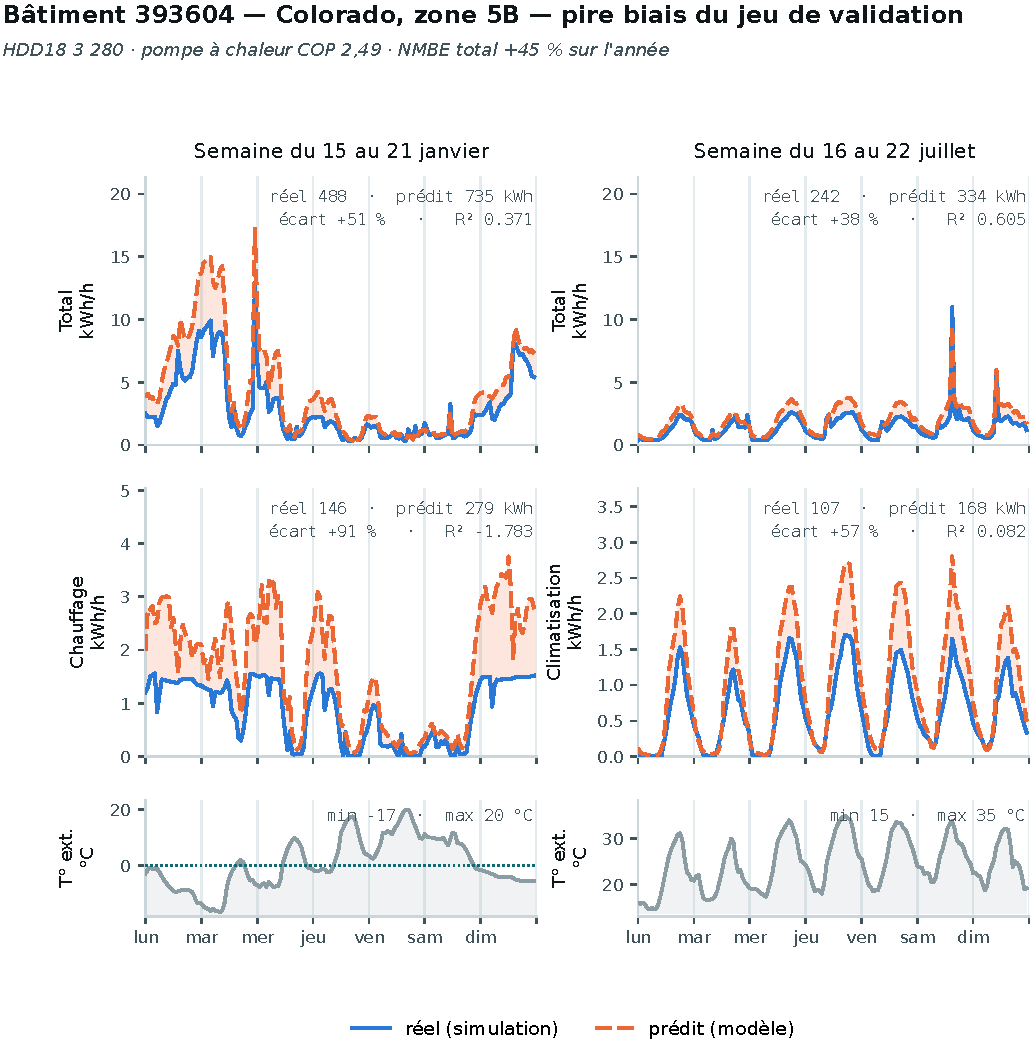
\includegraphics[height=0.72\textheight]{fig_courbe_393604.pdf}

\vspace{0.2em}
{\footnotesize Bâtiment 393604 --- Colorado, zone 5B, pompe à chaleur. La forme
journalière est correcte, le niveau du chauffage est doublé.}
\end{frame}

% ==================== 16 ====================
\begin{frame}{Ce qui a vraiment compté}
\vspace{0.2em}
\centering
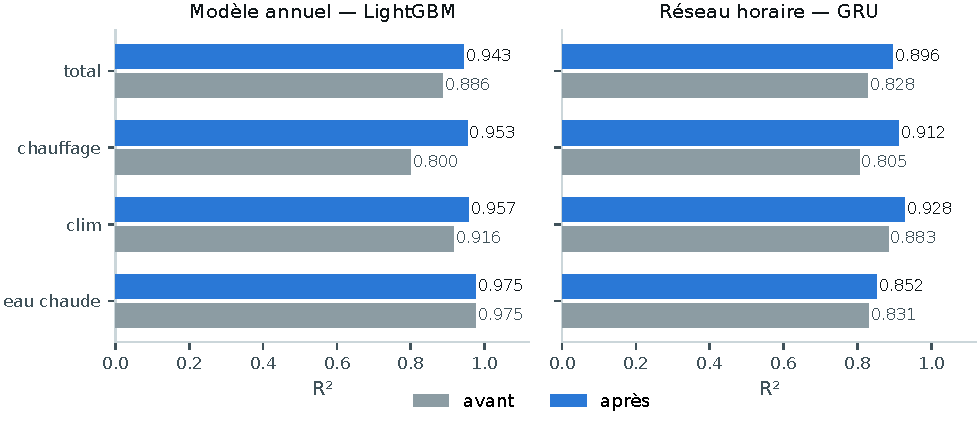
\includegraphics[width=0.68\linewidth]{fig_gains.pdf}

\vspace{0.5em}
\begin{columns}
\begin{column}{0.47\textwidth}\centering
\colorbox{VertOK}{\parbox{0.95\textwidth}{\centering\vspace{0.3em}\footnotesize
$4\times$ plus de \textbf{bâtiments}\\
503 $\rightarrow$ 2 005 : $\mathbf{+0{,}043}$\vspace{0.3em}}}
\end{column}
\begin{column}{0.47\textwidth}\centering
\colorbox{RougeFaible}{\parbox{0.95\textwidth}{\centering\vspace{0.3em}\footnotesize
$7\times$ plus de \textbf{fenêtres}\\
mêmes bâtiments : $\mathbf{+0{,}000}$\vspace{0.3em}}}
\end{column}
\end{columns}

\vspace{0.6em}
{\small Ce qui manquait n'était ni la capacité, ni le nombre d'heures, mais la
\textbf{diversité de bâtiments}.}
\end{frame}

% ==================== 17 ====================
% MAJ : le titre annonçait onze pistes pour huit lignes. Les onze y sont.
\begin{frame}{Onze pistes, mesurées une par une}
\vspace{0.2em}
\centering\footnotesize
\renewcommand{\arraystretch}{1.12}
\begin{tabular}{@{}p{5.9cm} r p{4.6cm}@{}}
\rowcolor{BleuFonce}
\textcolor{white}{\textbf{Piste}} & \textcolor{white}{\textbf{Effet}} &
\textcolor{white}{\textbf{Lecture}} \\
\rowcolor{GrisLeger} Tête multiplicative --- forme $\times$ niveau & $-0{,}027$ &
Déplace la difficulté vers une information absente \\
Cible en $\log(1+x)$ & $-0{,}015$ & Déplace l'erreur vers les gros consommateurs \\
\rowcolor{GrisLeger} GRU à 2 couches + dropout & $-0{,}009$ & Le plafond n'est pas
la capacité \\
FiLM --- modulation par le statique & $-0{,}008$ & La concaténation suffisait \\
\rowcolor{GrisLeger} Apports solaires $A_{\text{sol}} \times$ GHI & $-0{,}008$ &
Le rayonnement est déjà dans $f(t)$ \\
Moyennes glissantes de température & $-0{,}007$ & L'inertie est portée par le GRU \\
\rowcolor{GrisLeger} Objectif tweedie sur l'eau chaude & $-0{,}003$ & N'aide que
les cibles zéro-gonflées \\
Perte de Huber + pas adaptatif & $-0{,}002$ & --- \\
\rowcolor{GrisLeger} Fenêtres glissantes, \textit{stride} 24 & $+0{,}000$ &
Mêmes bâtiments \\
Produit enveloppe $\times$ écart & $+0{,}002$ & Le réseau le construit déjà \\
\rowcolor{VertOK} Climat dans le vecteur statique & $+0{,}008$ & Décisif pour
LightGBM, redondant ici \\
\end{tabular}

\vspace{0.5em}
{\small \textbf{Ajouter de la structure ne remplace pas l'information manquante.}}
\end{frame}

% ==================== 18 ====================
% NOUVELLE DIAPO — une anomalie trouvée dans les données, non documentée.
\begin{frame}{Une anomalie trouvée dans les données}
\vspace{0.2em}
\centering
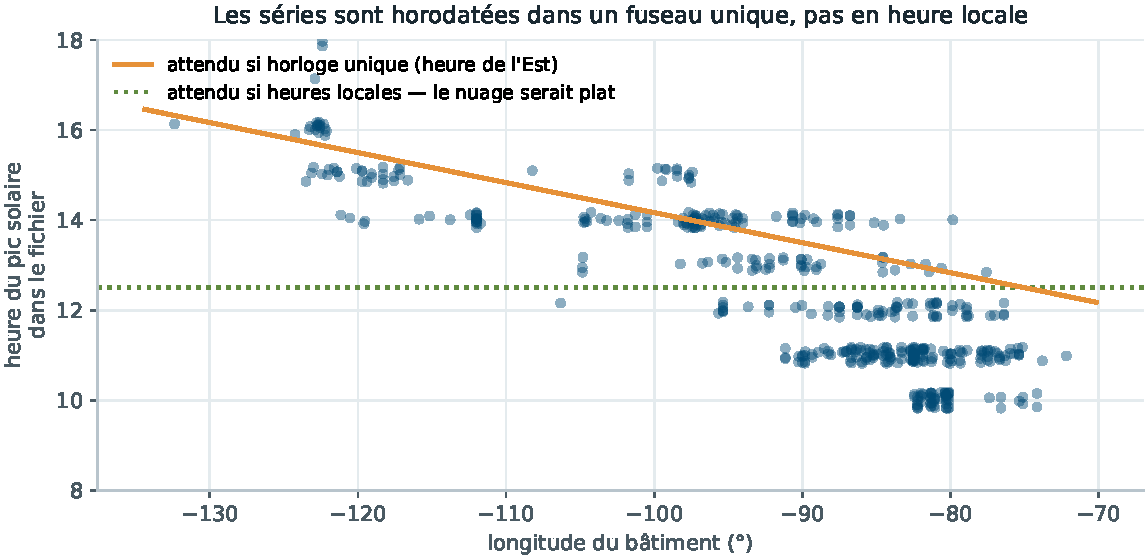
\includegraphics[width=0.82\linewidth]{fuseau_horaire.png}

\vspace{0.4em}
\begin{itemize}\setlength{\itemsep}{0.3em}
  \item Les séries sont horodatées dans un \textbf{fuseau unique} pour tout le
  pays, et non en heure locale
  \item Vérifié bâtiment par bâtiment contre les fichiers météo de comté :
  \textbf{3 heures} d'écart exactement en Californie
  \item Conséquence : une fenêtre « 18--21 h » visait \textbf{15--18 h} locales
  et manquait la pointe du soir
\end{itemize}
\end{frame}

% ==================== 19 ====================
\begin{frame}{Mesurer par différence}
\vspace{0.3em}
\centering
\begin{tikzpicture}[scale=0.9, transform shape, node distance=0.35cm and 0.6cm]
\node[etape, text width=2.2cm] (b1) {Bâtiment};
\node[etapeo, below=0.8cm of b1, text width=2.2cm] (b2) {Consigne décalée $-2$\,°C};
\node[final, right=of b1, text width=1.7cm] (m1) {Modèle};
\node[final, right=of b2, text width=1.7cm] (m2) {Même modèle};
\node[etape, right=of m1, text width=2.0cm] (c1) {Courbe de référence};
\node[etapeo, right=of m2, text width=2.0cm] (c2) {Courbe contrefactuelle};
\node[final, right=of c1, yshift=-0.8cm, text width=2.0cm] (d) {\textbf{Effacement}};
\draw[fl] (b1)--(m1); \draw[fl] (m1)--(c1);
\draw[fl] (b2)--(m2); \draw[fl] (m2)--(c2);
\draw[fl] (c1.east) -- ++(0.2,0) |- (d.west);
\draw[fl] (c2.east) -- ++(0.2,0) |- (d.west);
\end{tikzpicture}

\vspace{0.9em}
{\small\centering Aucun effacement n'est mesuré : il est \textbf{déduit} de
l'écart entre deux évaluations du même modèle.\par}

\vspace{0.6em}
\encadre[RougeFaible]{\small La consigne apparaît dans \textbf{quatre} colonnes
d'entrée. Les décaler toutes ensemble --- sinon on présente au réseau un logement
physiquement incohérent.}
\end{frame}

% ==================== 20 ====================
% NOUVELLE DIAPO — l'image qui rend l'effacement concret.
\begin{frame}{À quoi ressemble un effacement}
\vspace{0.3em}
\centering
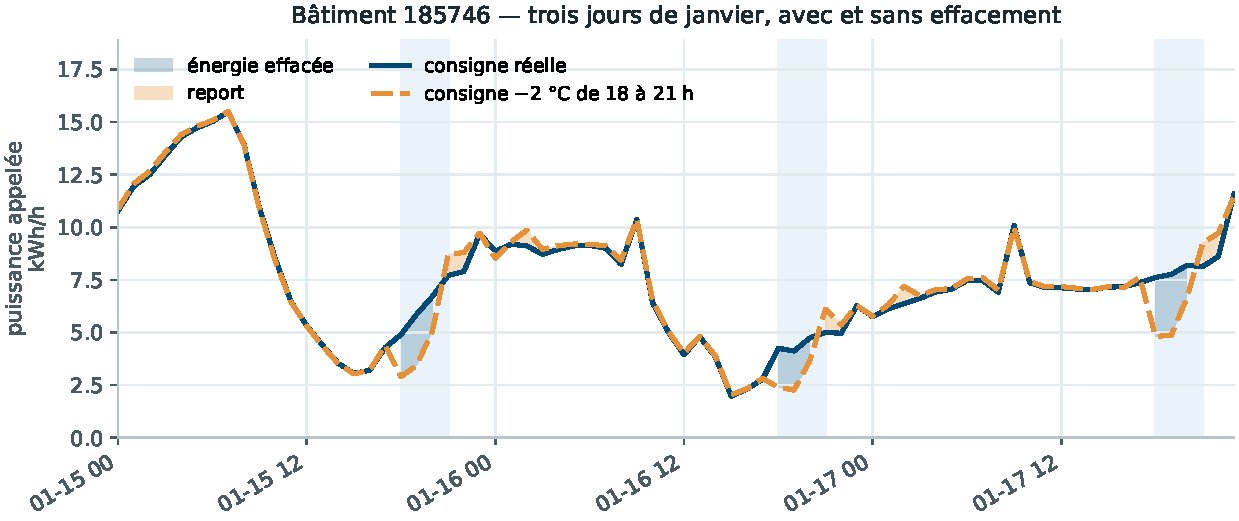
\includegraphics[width=0.92\linewidth]{flex_avant_apres.png}

\vspace{0.4em}
{\small Trois jours de janvier. Le creux pendant la fenêtre, la bosse de
\textbf{report} juste après.}
\end{frame}

% ==================== 21 ====================
% MAJ : 0,54 kWh/h venait de l'ancien scénario CLIMATISATION d'été, sur un modèle
% depuis abandonné. Valeurs mesurées sur le modèle actuel.
\begin{frame}{Le gisement, sur les 101 bâtiments de validation}
\vspace{0.2em}
\centering
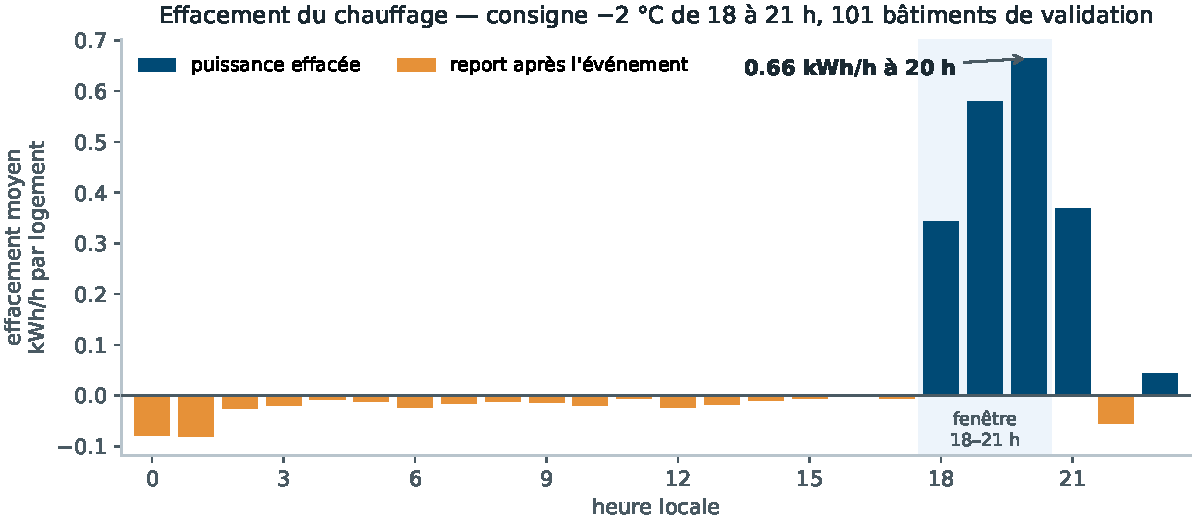
\includegraphics[width=0.86\linewidth]{profil_flexibilite.png}

\vspace{0.3em}
\begin{columns}
\begin{column}{0.31\textwidth}\centering
\colorbox{VertOK}{\parbox{0.95\textwidth}{\centering\vspace{0.3em}\footnotesize
\textbf{2,38 kW}\\pointe médiane\vspace{0.3em}}}
\end{column}
\begin{column}{0.31\textwidth}\centering
\colorbox{VertOK}{\parbox{0.95\textwidth}{\centering\vspace{0.3em}\footnotesize
\textbf{90 kWh}\\effacés sur l'hiver\vspace{0.3em}}}
\end{column}
\begin{column}{0.31\textwidth}\centering
\colorbox{BleuClair}{\parbox{0.95\textwidth}{\centering\vspace{0.3em}\footnotesize
\textbf{$-11$ \%}\\de report\vspace{0.3em}}}
\end{column}
\end{columns}

\vspace{0.4em}
{\footnotesize Report négatif : la nuit qui suit ne demande pas de remontée en
température.}
\end{frame}

% ==================== 22 ====================
% NOUVELLE DIAPO — résultat actionnable.
\begin{frame}{Jusqu'où peut-on pousser ?}
\vspace{0.2em}
\centering
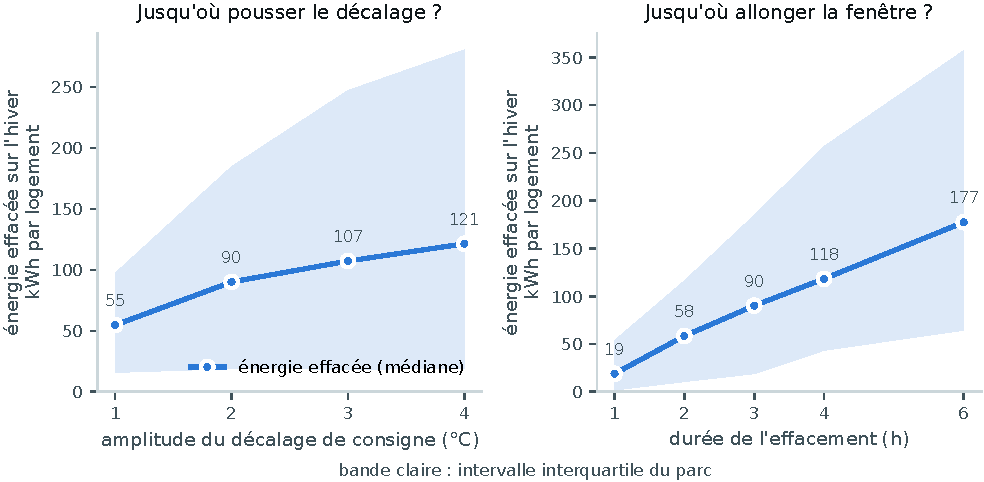
\includegraphics[width=0.88\linewidth]{fig_flex_reponse.pdf}

\vspace{0.4em}
\encadre[VertOK]{\small L'amplitude \textbf{sature} --- le chauffage est déjà à
l'arrêt. La durée reste \textbf{linéaire}.\\[0.2em]
Allonger la fenêtre vaut mieux que creuser la consigne, et gêne moins l'occupant.}
\end{frame}

% ==================== 23 ====================
\begin{frame}{Ce que valent ces chiffres}
\vspace{0.4em}
\begin{itemize}\setlength{\itemsep}{0.8em}
  \item \textbf{Test négatif} --- la consigne de chauffage décalée en \emph{été} :
  effet mesuré sur l'hiver \textbf{$-0{,}000$ kWh}. Le modèle n'invente pas
  d'effacement là où la physique l'interdit
  \item \textbf{Test d'identité} --- à décalage nul, la prédiction est inchangée
  au millionième de kWh
  \item \textbf{Cohérence physique} --- le signe est celui attendu, mais la
  corrélation avec les déperditions ($+0{,}17$) et l'inertie ($+0{,}12$) reste
  \textbf{faible}
\end{itemize}

\vspace{0.8em}
\encadre[JauneMoy]{\small Le gisement est très concentré --- \textbf{30 \% des
logements en portent 52 \%} ---\\
mais on ne sait pas encore \textbf{lesquels} à partir de leurs seules
caractéristiques. C'est la limite actuelle.}
\end{frame}

% ==================== 24 ====================
% MAJ : 503 -> 2 005 bâtiments.
\begin{frame}{Périmètre et perspectives}
\begin{columns}[T]
\begin{column}{0.47\textwidth}
\textbf{Ce sur quoi les résultats valent}
\vspace{0.6em}
\begin{itemize}\setlength{\itemsep}{0.6em}
  \item \textbf{2 005} maisons tout-électriques du parc \textbf{américain}
  \item Le confort n'est pas vérifié : le modèle ne prédit pas la température
  intérieure, d'où la borne à $\pm 2$\,°C
\end{itemize}
\end{column}
\begin{column}{0.47\textwidth}
\textbf{Suites}
\vspace{0.6em}
\begin{itemize}\setlength{\itemsep}{0.6em}
  \item La \textbf{climatisation}, protocole symétrique
  \item L'\textbf{eau chaude} : le ballon est un stock, mais sa consigne n'est
  pas dans les entrées
  \item Le \textbf{foisonnement} : décaler les groupes pour éviter un rebond
  synchronisé
  \item Transposer au parc français
\end{itemize}
\end{column}
\end{columns}
\end{frame}

% ==================== 25 ====================
\begin{frame}{Ce que j'en retiens}
\vspace{1em}
\begin{itemize}\setlength{\itemsep}{1.1em}
  \item Le \textbf{protocole d'évaluation} compte autant que le modèle
  \item Un \textbf{regard métier} sur les données change les résultats plus que
  le réglage du modèle
  \item Sur une chaîne partagée, les erreurs \textbf{ne s'annoncent pas} --- il
  faut des contrôles qui échouent bruyamment
\end{itemize}

\vspace{2em}
\begin{center}
{\Large\color{BleuFonce} Merci de votre attention}
\end{center}
\end{frame}

% =====================================================================
%  DIAPOS DE SECOURS — à garder après « Merci », pour les questions.
% =====================================================================

\begin{frame}{Annexe --- où se concentre le gisement}
\centering
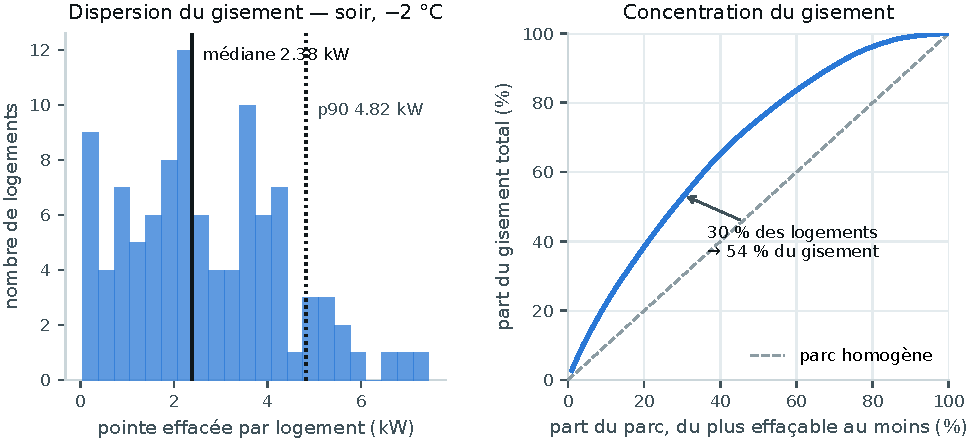
\includegraphics[width=0.9\linewidth]{fig_flex_distribution.pdf}
\end{frame}

\begin{frame}{Annexe --- deux autres bâtiments}
\begin{columns}[T]
\begin{column}{0.49\textwidth}\centering
{\scriptsize\textbf{170214} --- Colorado 7B, résistance}
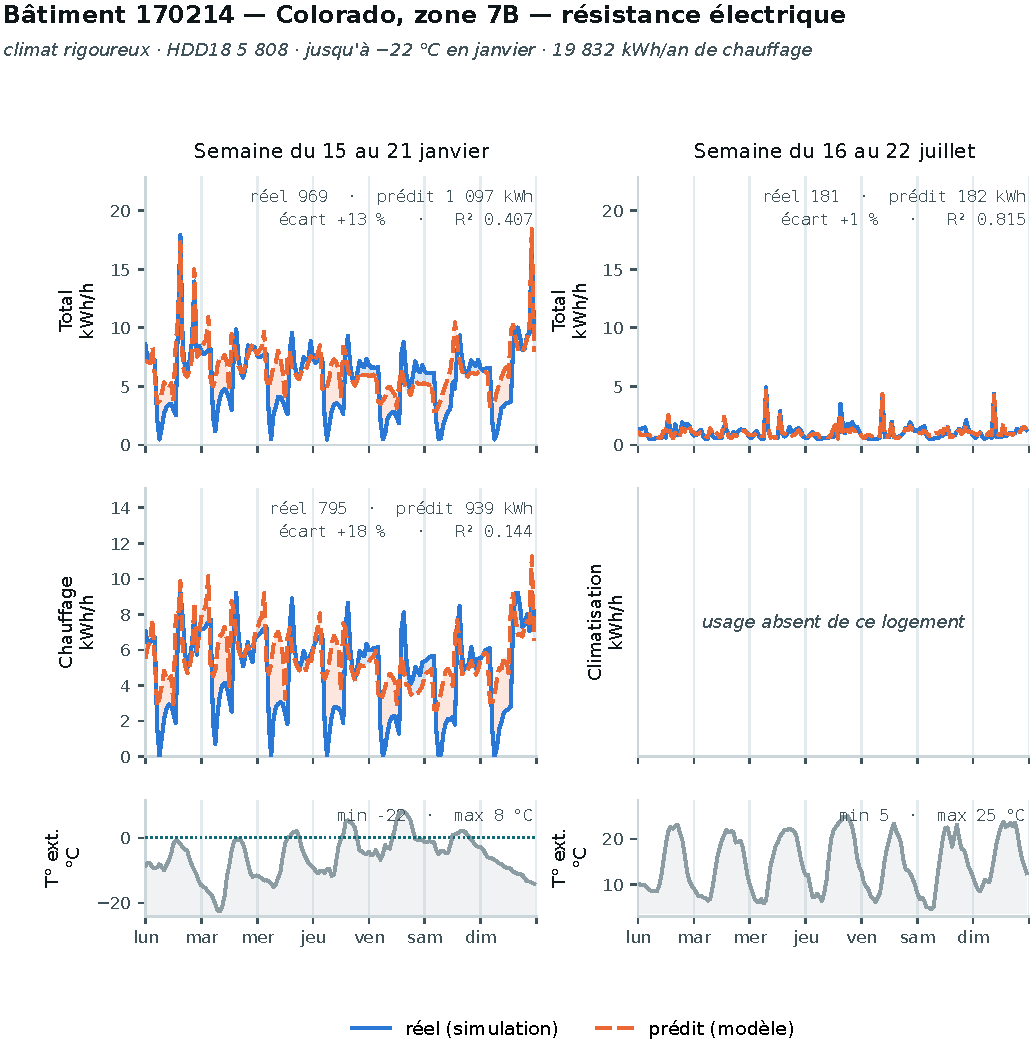
\includegraphics[width=\linewidth]{fig_courbe_170214.pdf}
\end{column}
\begin{column}{0.49\textwidth}\centering
{\scriptsize\textbf{420474} --- Arizona 2B, pompe à chaleur}
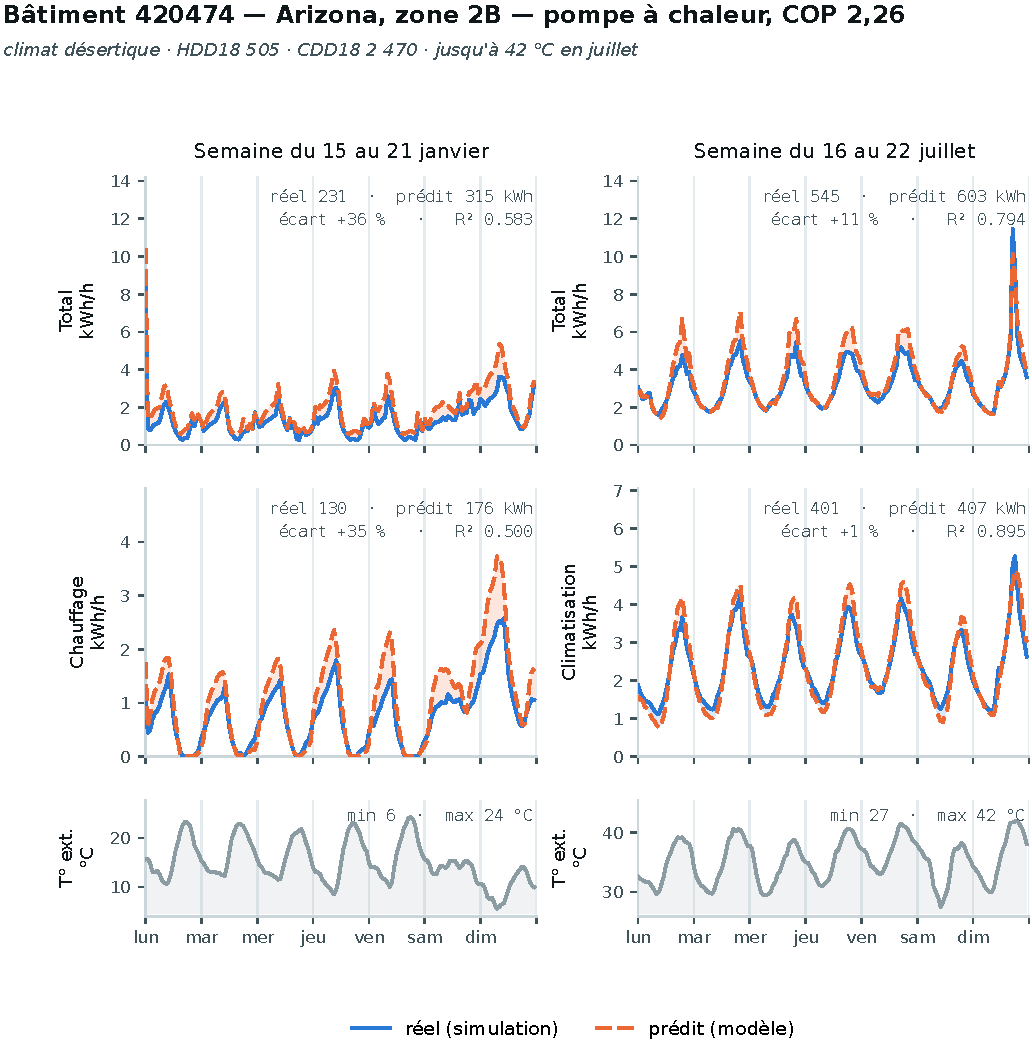
\includegraphics[width=\linewidth]{fig_courbe_420474.pdf}
\end{column}
\end{columns}
\end{frame}

\begin{frame}{Annexe --- un objectif adapté à chaque usage}
\vspace{0.4em}
\centering\small
\renewcommand{\arraystretch}{1.3}
\begin{tabular}{@{}l c c l@{}}
\rowcolor{BleuFonce}
\textcolor{white}{\textbf{Usage}} & \textcolor{white}{\textbf{$\ell_2$}} &
\textcolor{white}{\textbf{Tweedie}} & \textcolor{white}{\textbf{Retenu}} \\
\rowcolor{GrisLeger} Total & 0,9408 & 0,9408 & $\ell_2$ \\
Chauffage & 0,9453 & \textbf{0,9526} & \cellcolor{VertOK}Tweedie \\
\rowcolor{GrisLeger} Climatisation & 0,9503 & \textbf{0,9550} &
\cellcolor{VertOK}Tweedie \\
Eau chaude & \textbf{0,9738} & 0,9714 & \cellcolor{JauneMoy}$\ell_2$ \\
\end{tabular}

\vspace{0.8em}
{\small Le chauffage est \textbf{zéro-gonflé} : beaucoup de logements du Sud à
exactement 0, les autres jusqu'à 85\,000 kWh/an. Tweedie modélise ce cas ---
une masse en zéro plus une queue continue positive. Appliqué \textbf{par usage},
pas en bloc.}
\end{frame}

\end{document}
